\documentclass{./../div_teaching_slides}

\begin{document}
\title{ECON 340 \\ Economic Research Methods}
\author{Div Bhagia}
\date{Lecture 24 \\ Differences-in-Differences \& Event Study Designs}


%%%%%%%%%%%% 
\begin{frame}[noframenumbering, plain]
\maketitle
\end{frame}

%%%%%%%%%%%%%%%%%%%%
\begin{frame}{Answers to Causal Questions}
\begin{witemize}
  \item Lots of important questions in economics are of a causal nature. 
  \item For example --- what is the impact of immigration on labor markets? Or how do minimum wages impact employment?
  \item Experiments are the gold standard, but not always feasible. 
  \item So we look for natural experiments. 
\end{witemize}
\end{frame}


%%%%%%%%%%%%%%%%%%%%
\begin{frame}{Differences-in-Differences Estimator}
\begin{witemize}
  \item Two groups: Treatment ($T$) and Control ($C$)
  \item Two time-periods: Pre ($t=0$) and Post ($t=1$)
  \item Differences-in-Differences (DID) estimator:
 \begin{align*}
  	\beta_1^{DID} &= (\bar{Y}^T_1 - \bar{Y}^T_0)-(\bar{Y}^C_1 - \bar{Y}^C_0) 
  	\\[0.5em] 
  	& = \Delta \bar{Y}^T - \Delta \bar{Y}^C
  \end{align*}
  where $\Delta \bar{Y}^T$ and $\Delta \bar{Y}^C$ is the average change in $Y$ in the treatment and control group, respectively. 
\end{witemize}
\end{frame}

%%%%%%%%%%%%%%%%%%%%
\begin{frame}{Differences-in-Differences}
\pgfplotsset{compat=newest, width=12cm, height=8cm}
\centering
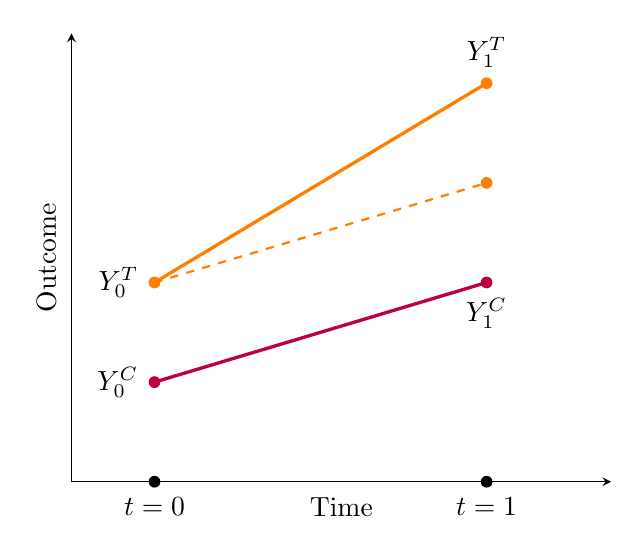
\begin{tikzpicture}
\begin{axis}[
    axis lines = left,
    xlabel = Time,
    ylabel = Outcome,
    xtick=\empty,
    ytick=\empty,
    clip=false,
    xmin=0, xmax=13,
    ymin=0, ymax=9
]
% Points
\node[label={180:{$Y^C_{0}$}},circle,fill,inner sep=1.5pt,purple] at (axis cs:2,2) {};
\node[label={-90:{$Y^C_{1}$}},circle,fill,inner sep=1.5pt, purple] at (axis cs:10,4) {};
\node[label={180:{$Y^T_{0}$}},circle,fill,inner sep=1.5pt, orange] at (axis cs:2,4) {};
\node[label={90:{$Y^T_{1}$}},circle,fill,inner sep=1.5pt, orange] at (axis cs:10,8) {};
\node[circle,fill,inner sep=1.5pt, orange] at (axis cs:10,6) {};
% Lines
\addplot [purple, no marks, very thick] coordinates {(2,2) (10,4)};
\addplot [orange, no marks, very thick] coordinates {(2,4) (10,8)};
\addplot [orange, dashed, no marks, thick] coordinates {(2,4) (10,6)};
% Time points
\node[label={-90:{$t=0$}}, circle, fill,inner sep=1.5pt] at (axis cs:2,0) {};
\node[label={-90:{$t=1$}}, circle, fill,inner sep=1.5pt] at (axis cs:10,0) {};
\end{axis}
\end{tikzpicture}
\end{frame}

%%%%%%%%%%%%%%%%%%%%
\begin{frame}{Mariel Boatlift}
\begin{witemize}
  \item In April 1980, Fidel Castro unexpectedly allowed all Cubans
who wished to leave the country to do so from the port of Mariel. 
\item Around 50\% of these immigrants settled in Miami.
\item This led to a 7\% increase in the labor force of Miami. 
\item Card (1990) studies the impact of the Boatlift on the Miami labor market by comparing wage and employment trends in Miami with those in four comparison cities. 
\end{witemize}
\end{frame}

%%%%%%%%%%%%%%%%%%%%
\begin{frame}{Card and Krueger (1994)}
\vspace{-0.5em}
April 1, 1992: Hourly minimum wage in New Jersey increased from \$4.25 to \$5.05 \\  \vspace{0.25em}
\centering
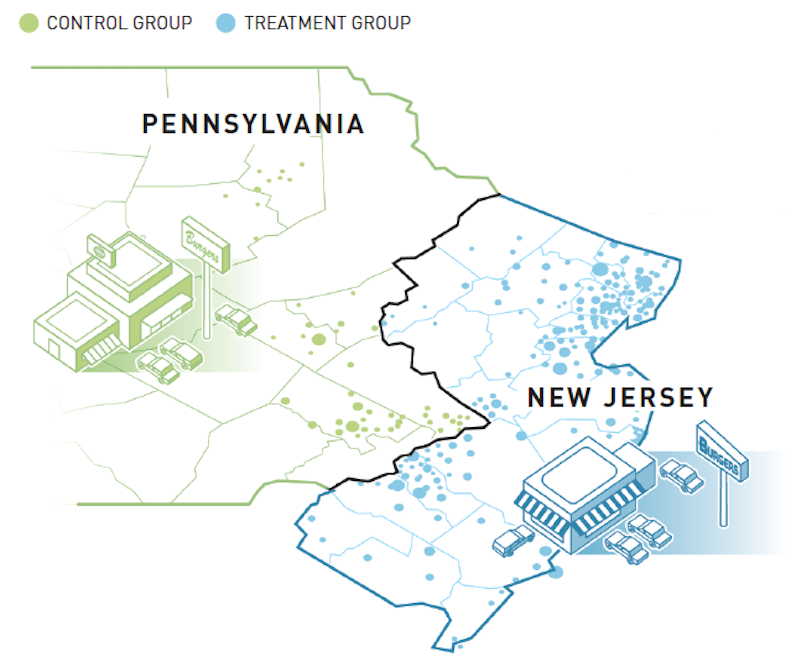
\includegraphics[scale=0.3]{treatment-control-group.png}
\end{frame}


%%%%%%%%%%%%%%%%%%%%
\begin{frame}{Observed Outcomes}
\pgfplotsset{compat=newest, width=12cm, height=8cm}
\centering
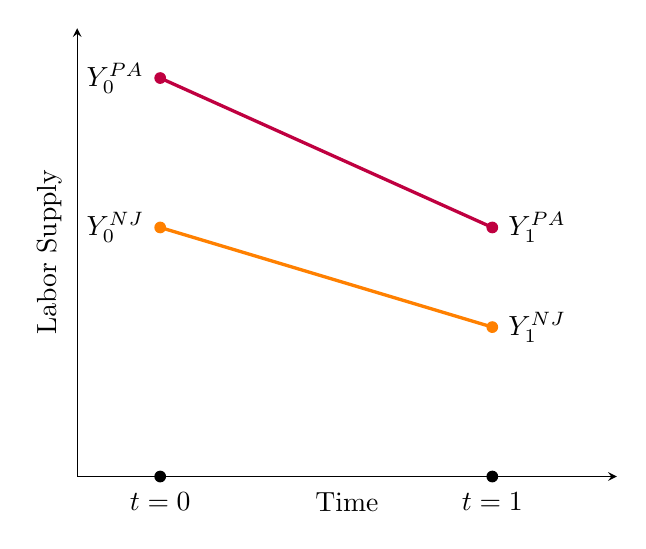
\begin{tikzpicture}
\begin{axis}[
    axis lines = left,
    xlabel = Time,
    ylabel = Labor Supply,
    xtick=\empty,
    ytick=\empty,
    clip=false,
    xmin=0, xmax=13,
    ymin=0, ymax=9
]
% Points
\node[label={180:{$Y^{NJ}_{0}$}},circle,fill,inner sep=1.5pt,orange] at (axis cs:2,5) {};
\node[label={0:{$Y^{NJ}_{1}$}},circle,fill,inner sep=1.5pt, orange] at (axis cs:10,3) {};
\node[label={180:{$Y^{PA}_{0}$}},circle,fill,inner sep=1.5pt, purple] at (axis cs:2,8) {};
\node[label={0:{$Y^{PA}_{1}$}},circle,fill,inner sep=1.5pt, purple] at (axis cs:10,5) {};
%\node[circle,fill,inner sep=1.5pt, orange] at (axis cs:10,6) {};
% Lines
\addplot [orange, no marks, very thick] coordinates {(2,5) (10,3)};
\addplot [purple, no marks, very thick] coordinates {(2,8) (10,5)};
% Time points
\node[label={-90:{$t=0$}}, circle, fill,inner sep=1.5pt] at (axis cs:2,0) {};
\node[label={-90:{$t=1$}}, circle, fill,inner sep=1.5pt] at (axis cs:10,0) {};
\end{axis}
\end{tikzpicture}
\end{frame}

%%%%%%%%%%%%%%%%%%%%
\begin{frame}{Differences-in-Difference Design}
\begin{witemize}
  \item Say, labor supply declined in both states over this period due to seasonality or aggregate trends in the economy
  \item We might be tempted to attribute the decline in labor supply over this period in NJ to increased minimum wages (unintuitive!)
  \item Differences-in-Difference design: look at how labor supply evolved in NJ relative to the control group (PA)
\end{witemize}
\end{frame}

%%%%%%%%%%%%%%%%%%%%
\begin{frame}{Differences-in-Difference Estimator}
\pgfplotsset{compat=newest, width=12cm, height=8cm}
\centering
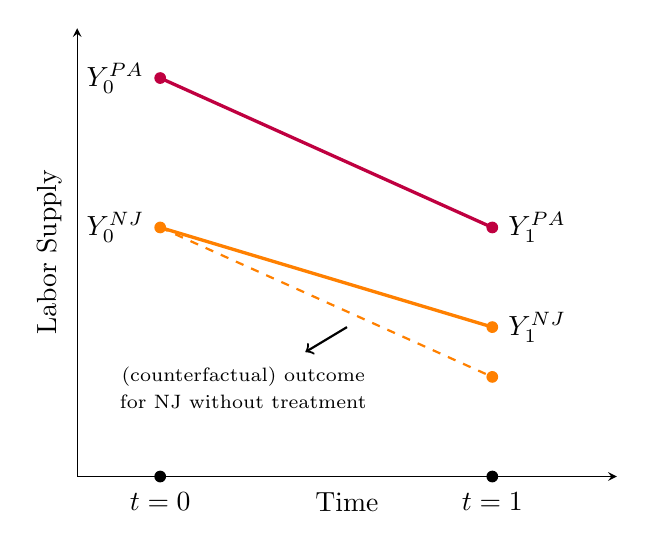
\begin{tikzpicture}
\begin{axis}[
    axis lines = left,
    xlabel = Time,
    ylabel = Labor Supply,	
    xtick=\empty,
    ytick=\empty,
    clip=false,
    xmin=0, xmax=13,
    ymin=0, ymax=9
]
% Points
\node[label={180:{$Y^{NJ}_{0}$}},circle,fill,inner sep=1.5pt,orange] at (axis cs:2,5) {};
\node[label={-0:{$Y^{NJ}_{1}$}},circle,fill,inner sep=1.5pt, orange] at (axis cs:10,3) {};
\node[label={180:{$Y^{PA}_{0}$}},circle,fill,inner sep=1.5pt, purple] at (axis cs:2,8) {};
\node[label={0:{$Y^{PA}_{1}$}},circle,fill,inner sep=1.5pt, purple] at (axis cs:10,5) {};
\node[circle,fill,inner sep=1.5pt, orange] at (axis cs:10,2) {};
% Lines
\addplot [orange, no marks, very thick] coordinates {(2,5) (10,3)};
\addplot [purple, no marks, very thick] coordinates {(2,8) (10,5)};
\addplot [orange, dashed, no marks, thick] coordinates {(2,5) (10,2)};
% Time points
\node[label={-90:{$t=0$}}, circle, fill,inner sep=1.5pt] at (axis cs:2,0) {};
\node[label={-90:{$t=1$}}, circle, fill,inner sep=1.5pt] at (axis cs:10,0) {};
% Arrow
\draw[->, thick] (axis cs:6.5,3) -- (axis cs:5.5,2.5); 
\node at (axis cs:4,2) {\scriptsize (counterfactual) outcome};
\node at (axis cs:4,1.5) {\scriptsize for NJ without treatment};
\end{axis}
\end{tikzpicture}
\end{frame}

%%%%%%%%%%%%%%%%%%%%
\begin{frame}{Differences-in-Difference Design}
\begin{witemize}
  \item Underlying assumption: parallel trends for treatment and control groups in the absence of treatment
  \item We are not saying outcomes are similar for NJ and PA, but just that they move similarly over time
  \item In practice, one can often test this assumption by looking at pre-trends
  \item Event-study designs: examine the difference in outcomes for two groups over a longer pre-period 
  \end{witemize}
\end{frame}


%%%%%%%%%%%%%%%%%%%%
\begin{frame}{Event Study Design}
\centering
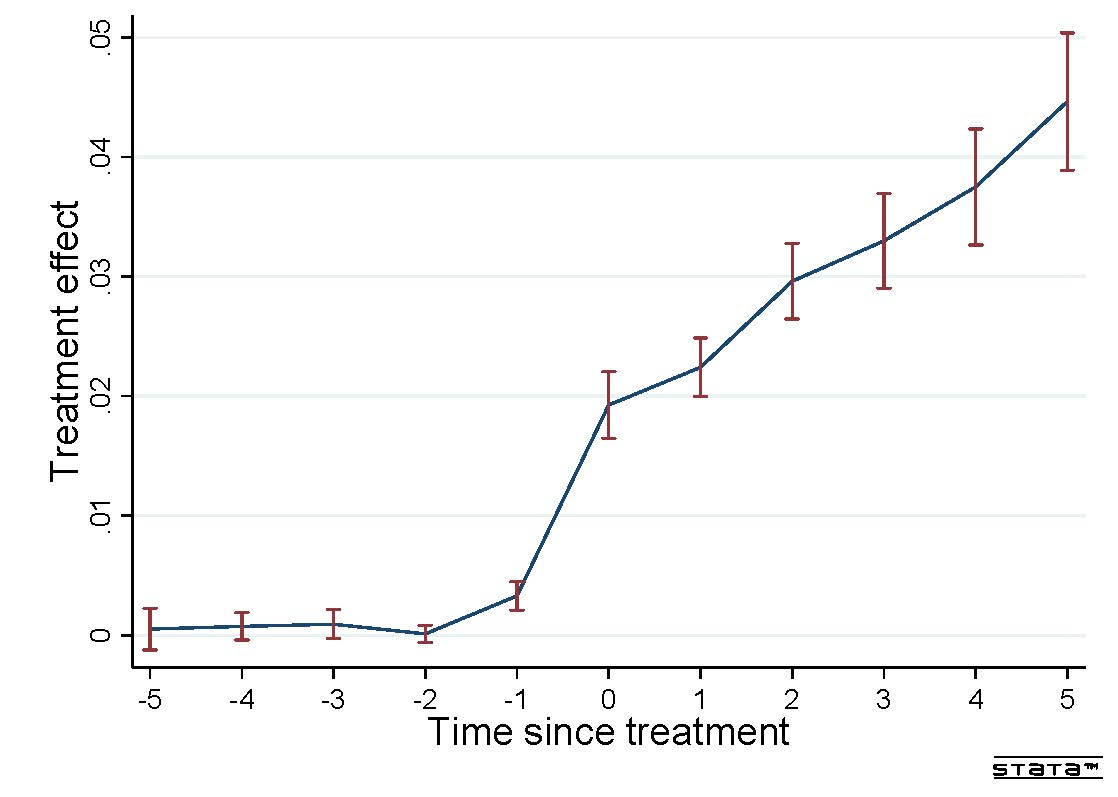
\includegraphics[scale=0.75]{event_study.jpeg}
\end{frame}

%%%%%%%%%%%%%%%%%%%%
\begin{frame}{Child Marriage in Mexico}
\centering
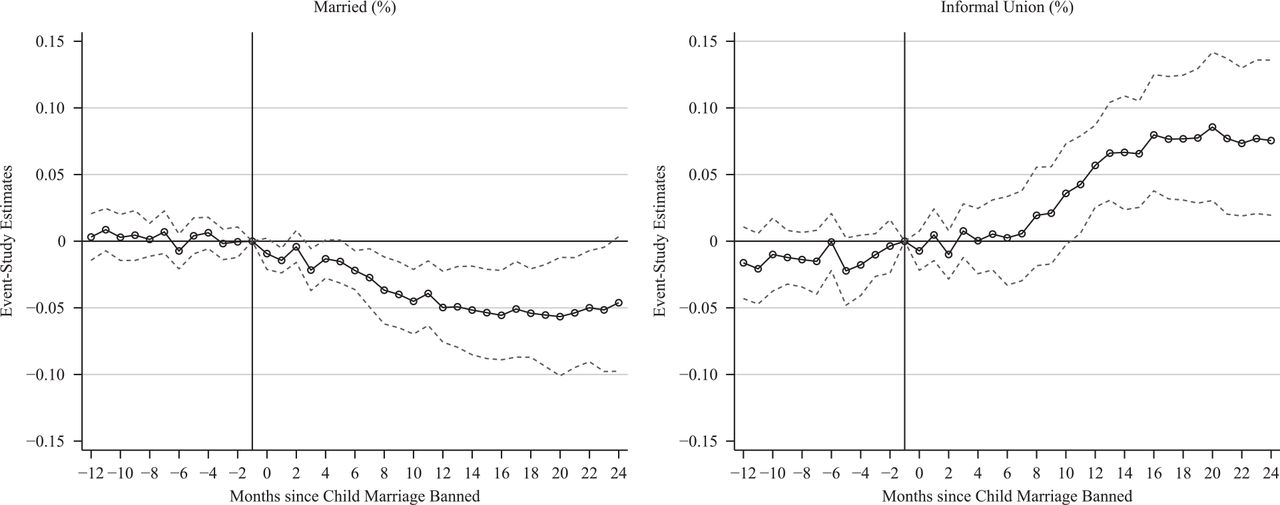
\includegraphics[scale=1.25]{eg1.jpg} \\~\\
Source: Belles-Obrero and Lombardi (2023)
\end{frame}

%%%%%%%%%%%%%%%%%%%%
\begin{frame}{Trade War}
\centering
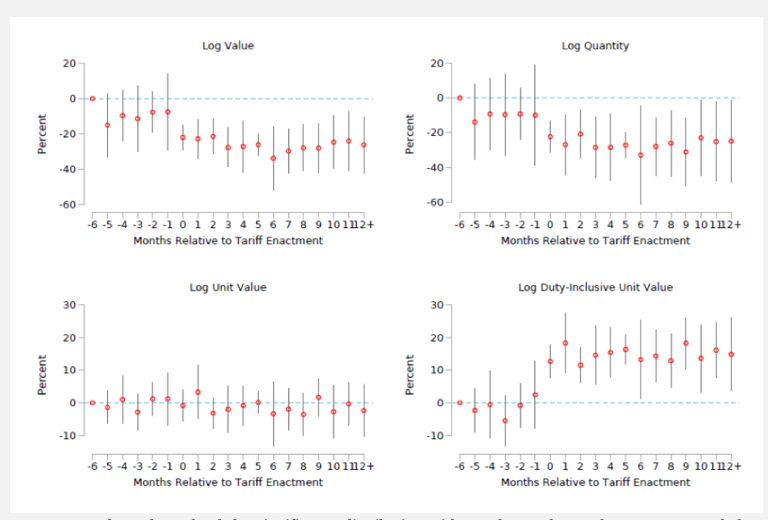
\includegraphics[scale=0.4]{eg2_1.png}
\end{frame}

%%%%%%%%%%%%%%%%%%%%
\begin{frame}{Trade War}
\centering
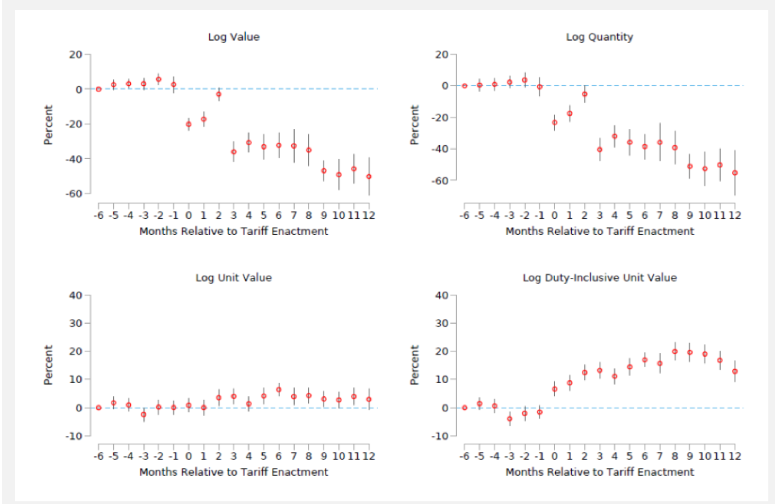
\includegraphics[scale=0.4]{eg2_2.png}
\end{frame}


%%%%%%%%%%%%%%%%%%%%
\begin{frame}{Taking Stock}
\begin{witemize}
 \item Link for reading: \href{https://microeconomicinsights.org/the-return-to-protectionism/}{https://microeconomicinsights.org/the-return-to-protectionism/}
  \item Research paper due next week Tues (12/05)
  \item Talk about Big Data \& Machine Learning on Tues
  \item Review class for the midterm on Thurs
  \item I won't be here to proctor your exam, but will be available to clarify in case something comes up
  \item Please fill the SOQs :)
\end{witemize}

\end{frame}



\end{document}